\documentclass[a4paper,11pt]{article}
\usepackage[utf8]{inputenc}
\usepackage{fullpage}
\usepackage{graphicx}
\usepackage{wrapfig}
\usepackage{caption}
\usepackage{subcaption}
\usepackage{appendix}
\usepackage{tcolorbox}
\tcbuselibrary{theorems}

\newtcbtheorem[number within=section]{theo}{}%
{colback=green!5,colframe=green!35!black,fonttitle=\bfseries}{th}

\usepackage{hyperref}
\definecolor{navyblue}{rgb}{0.0, 0.0, 0.5}
\definecolor{myblue}{RGB}{15,77,145}
\definecolor{mountainmeadow}{rgb}{0.19, 0.73, 0.56}
\hypersetup{
	colorlinks=true,
	linkcolor=myblue,
	citecolor=mountainmeadow,
	urlcolor=navyblue,
}

\title{% 
	4F13: Probabilistic Machine Learning \\
	\vspace{10pt}
	\small Summarized from C. Rasmussen \& D. Krueger lectures, Michaelmas 2021}
\author{\small Oussama Chaib}
\date{\small October 2021}

\begin{document}
	\maketitle
	\tableofcontents
	\pagebreak
	\section{Introduction}
	\subsection{Modelling data}
	\subsubsection{Purpose of models}
	The purpose of models is:
	\begin{itemize}
		\item Making predictions
		\item Generalizing: interpolation, extrapolation
		\item Generating more data from a similar distribution as the training set
		\item Compressing and summarizing data
		\item Interpreting statistical relationships in data
		\item Evaluating the relative probability of a hypothesis on data
	\end{itemize}
	\subsubsection{Origin of models}
	The origin of models can be:
	\begin{itemize}
		\item \textbf{First principles:}  (i.e: Newtonian mechanics model, high level of accuracy)
		\item \textbf{Observations and data:} (i.e: annual production of timber depending on climate and geographical factors)
	\end{itemize}
	\textbf{Definition --} Machine learning is a broad term that covers theory and practice of mathematical models which to a significant degree rely on data.
	\subsubsection{Priors}
	Every model relies on priors: 
	\begin{itemize}
		\item \textbf{Knowledge}
		\item \textbf{Assumptions} (could be true or false)
		\item \textbf{Simplifying assumptions} (not necessarily true, but good enough -- i.e:  the mistake associated with the assumption is fairly small even though it might not be necessarily true)
	\end{itemize}
	\subsubsection{Components of a model}
	Time series have: 
	\begin{itemize}
		\item Unobserved/hidden/latent variables ($x(t)$, $x(t-1)$)
		\item Observations (shaded $y(t)$, $y(t-1)$)
		\item Parameters to link everything 
		\begin{itemize}
			\item Transitions (between latent variables)
			\item Emissions (from a lantent variable to an observation)
		\end{itemize}
	\end{itemize}
	\underline{\emph{Note:}} The number of latent variables increases with the number of observations, but the number of parameters doesn't!\\
	\textbf{-- Learning/training models:} "What to do with all this data?"\\ Depending on the data, some models include: inference, estimation, sampling, and marginalization.
	\subsubsection{Practical modelling}
	\begin{enumerate}
		\item Treat (training) the unobserved quantities (latent variables, observations, parameters)
		\item Make predictions based on test cases, interpret the trained model (can we figure out what the model is trying to tell us about the data?)
		\item Evaluate the accuracy of the data
		\item Model selection and criticism (choose the right model or variant of the model, identify limitations)
	\end{enumerate}
	There is not "true" or "correct" model -- \emph{"All models are wrong, but some are useful"} - George E.T. Box
	\subsection{Linear in the parameters regression}
	Let's start off with a dataset $D={x_i,y_i}^N_{i=1}$. From a dataset of N points, we would like to infer the coordinate $y_*$ at $x_*$. A simple model to do that would be polynomial \textbf{linear in the parameters} regression:
	\[f_w(x)=w_0+w_1 x+w_2 x^2+...+w_M x^M\]
	where $w_i$ are the corresponding weights of the polynomial, and the \textbf{parameters} of the model.
	\vspace{5pt}\\
	\textbf{-- Relevant questions:}
	\vspace{5pt}\\
	\emph{Model structure:} Should we choose a polynomial? What degree $M$ should we choose?\\
	\emph{Parameters:} What values of $w_i$ do we choose?
	\subsubsection{Least squares approach}
	Let's find the "best" polynomial (degree $M$ and weights $w_i$) according to the least squares approach (minimizing the variance or sum of squared error $e_i^2$):
	\[e_i(x)^2=(y_i(x_i)-f_w(x_i))^2\]
	\[E(x)=\sum^N_{i=1} e_i^2\]
	\vspace{5pt}\\
	\underline{\textbf{-- Some notations:}}
	\begin{itemize}
		\item \textbf{Training target} (input data that we would like to fit):
		\[  y = [y_1,...,y_N]  \]
		\item \textbf{Prediction} (the functions that will attempt to fit the data $y$):
		\[  f = [f_w(x_1),...,f_w(x_N)]  \]
		\item \textbf{Errors}:
		\[  e = f-y = [e_1,...,e_N]  \]
		\item \textbf{Parameters (what we're solving for!):} The \textbf{weights} of $f$:
		\[ w = [w_0,...,w_M]  \]
	\end{itemize}
	The sum of errors we would like to minimize is (defined as a variance to minimize):
	\[ E(w) = ||e||^2 = e^Te= (f-y)^T(f-y)\]	
	We define the \textbf{basis function} of the model (linear in the parameters model) as a matrix that contains all the $x^j$ (the matrix contains a list of all polynomials of unknown $x$ with maximum order from 0 to M) :
	\[ \Phi = \Phi_{i,j} =  \begin{bmatrix}
		\phi_0(x_1) & ... & \phi_M(x_1)\\
		... & ... & ...\\
		\phi_0(x_M) & ... & \phi_M(x_M)
	\end{bmatrix}
	\]
	\begin{center}
		where $\phi_j(x) = x^j $
	\end{center}
Ultimately, we can define the prediction function as a \textbf{linear in parameters} model that is the product of the \emph{basis function} and the \emph{weights}:
\begin{center}
	\fbox{$f = \Phi . w$}
\end{center}
To minimize the sum of squared errors $E(w)$, the gradient of the function should be equal to the zero vector:
\[  \frac{\partial E(w)}{\partial w} = 2 \Phi^T \Phi w - 2 \Phi^Ty = "0" \]
The weight vector $\hat{w}$ that minimizes $E(w)$:
\begin{center}
	\fbox{$\hat{w} = (\Phi^T Phi)^{-1} \Phi^T y$}
\end{center}
\textbf{The error vector is \underline{minimal} when it orthogonal with all columns of $\Phi$:}
\[ \Phi^T.e = 0 \]
\begin{figure}[h]
	\centering
	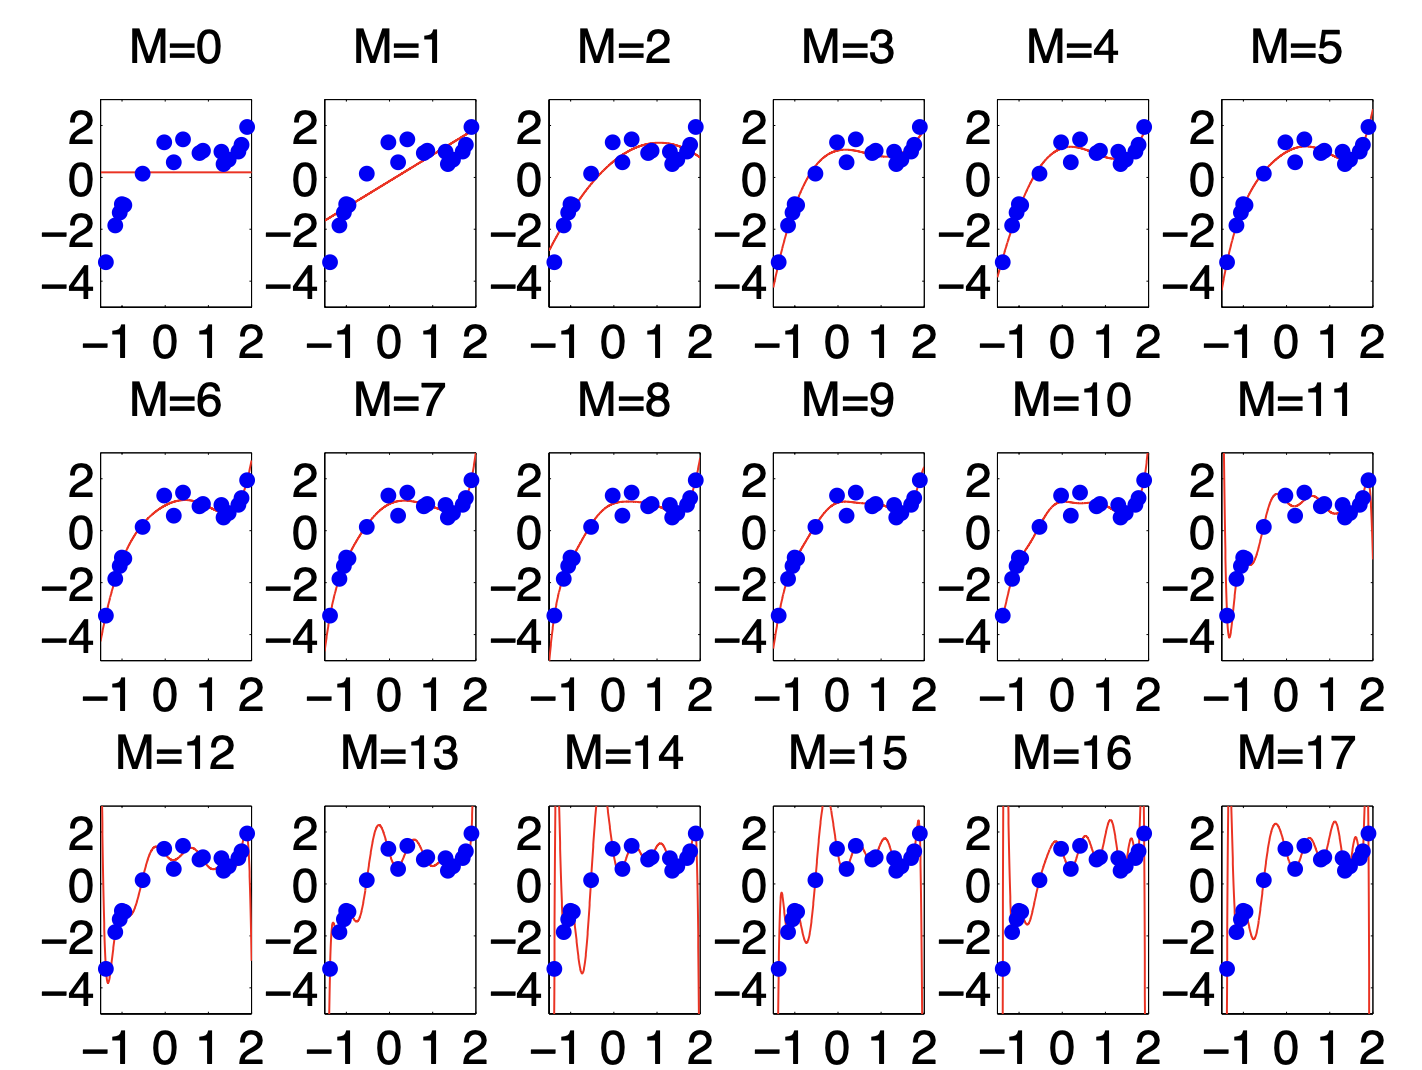
\includegraphics[width=.8\linewidth]{figures/M.png}
	\caption{Overfitting illustrated. In this example, we are solving for the \underline{weights} for each case of M}
\end{figure}
When we go to higher values of M, we are able to fit a function that minimizes the error term but we may run into the problem of \textbf{overfitting}. In that case, \textbf{additional assumptions} are needed.
\subsubsection{Probabilistic approach: Likelihood and concept of noise}
\textit{(Probabilistic view of what was done in the previous section. We're doing the exact same thing but using probabilities, only to end up getting equivalent weights)}\vspace{5pt}\\
\underline{\textbf{Definition:}} The \textbf{likelihood} is the probability of the data given the parameters.\vspace{5pt}\\
\textit{Example:}
\begin{itemize}
	\item $p(y|w,\sigma^2)$ is the probability of the observed data given the weights and noise.
	\item $L(w) \propto p(y|w,\sigma^2)$ is the \textbf{likelihood} of the weights.
\end{itemize}
The \textbf{maximum likelihood} of the weights:
\[ \hat{w} = argmax(L(w)) = argmax(e^{-\frac{E(w)}{2 \sigma_noise^2}}) = argmin(E(w)) \]
which is equivalent to the result that we got using least squares. But we still haven't solved the problem: we still overfit!
	\subsection{Comments from QnA}
	-- Why is the error vector $e$ minimal if it's orthogonal to all columns of $\phi$?\vspace{3pt}\\
	$\phi$ is a fixed function, it doesn't have any parameters in it. Still linear in parameters because the product of $w$ and $\phi$ matrices is linear (even at high polynomial orders).\vspace{5pt}\\
	-- What is Euclidian geometry?\vspace{3pt}\\
	Simple geometries, straight lines, basic shapes (including circle).\vspace{5pt}\\
	-- Bayesian methods, why are they not as popular?\vspace{3pt}\\
	Not so sure about that. Maximum likelihood (used often, single value that best explains the data, quite popular/successful).
\end{document}